\documentclass[border=4pt]{standalone}
\usepackage{amsmath}
\usepackage{tikz}
\usetikzlibrary{arrows.meta,positioning}
\begin{document}
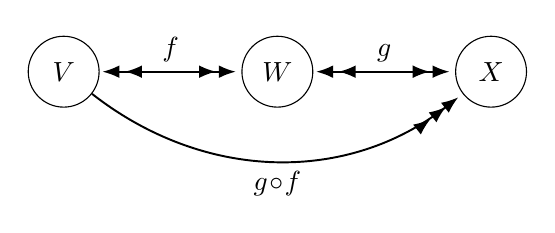
\begin{tikzpicture}[
  node distance=18mm,
  object/.style={draw,circle,minimum size=9mm,inner sep=1pt},
  morphism/.style={line width=.7pt,
    {Latex[sep=1pt] Latex[sep=2pt]}-{Latex[sep=1pt] Latex[sep=2pt]}}
]
  \node[object] (V) {$V$};
  \node[object,right=of V] (W) {$W$};
  \node[object,right=of W] (X) {$X$};

  \draw[morphism] (V) -- node[above] {$f$} (W);
  \draw[morphism] (W) -- node[above] {$g$} (X);
  \draw[line width=.7pt,-{Latex[sep=1pt] Latex[sep=-.5pt] Latex[sep=2pt]}]
    (V) to[bend right=38] node[below] {$g\!\circ\! f$} (X);
\end{tikzpicture}
\end{document}
